
The generative model used to generative grasps, explained in the previous section, works with a partial cloud with no assumptions about the object's weight, model, or friction parameters. In a fashion similar to \cite{Levine1}, it is possible to perform the generated grasps and record the outcome. The collective set of grasps and outcomes in simulation, accompanied with corresponding depth images, can be used to train a neural network that can predict whether new image, grasp pairs will succeed or not. This is the approach employed in this paper. 

It is time-consuming and expensive to collect real grasp data with using robotic arms with dexterous hands. Unlike gripper + arm combinations which require relatively less supervision \cite{Levine1}, dexterous hands can be much more fragile due to their complexity. Advances in physics simulators have made it possible to re-create robotic experiment setups in simulation. We created a simulated experimental setup in order evaluate grasp, which allowed us to collect as much data as needed in a short period of time with no supervision.

In this section, we discuss the architecture of our grasp predictor network $f(I_t, h_t)$, where $I^t$ stands for a colorized depth image of the object, and $h_t = (h_{tw}, h_{tc})$ is the grasp parameters with respect to the camera used to acquire the depth image. The network outputs a grasp success probability between $[0,1]$ for any image $I_t$ and grasp $h_t$ pair. The reader is advised to refer to Section \ref{section:simulation} for details of data collection in simulation.

Our network architecture is given in Figure~\ref{fig:networkArchitecture}. The purpose of the network is to learn the relationship between the point cloud, given as a colorized depth image, and grasp (hand shape) parameters which encode the configuration of the hand with respect to the camera frame. This is a complex task, as the kinematic model of the hand is unknown to the network, and it has to consider each grasp as a black box: The network knows the inputs that configure the hand, including the joint positions, and only has access to the outcome in the form of success/failure. Implementation-wise, our network combines a version of VGG-16 network with inherited weights from training on ImageNet, with fully connected layers consisting of 1024 nodes each, followed by RELU layers. 
% Talk more about the architecture

The Depth image colorization employed in our paper is an operation that takes a 1-channel depth image $I_{t}^{depth}$ and produces a 3-channel image $I_t$ that can be directly given as input to the VGG-16 network. First, the $640 \times 480$ depth image is cropped by a square window of size $460 \times 460$, located in the center of the image. Then, it is down-sampled to an image of size $224 \times 224$. The colorization process creates a $224 \times 224$ 3-channel image, where the first two channels of the output image $I_t$ are simplified mean curvature and simplified Gaussian curvature, respectively. The formula of mean curvature is $h = {gr}_{xx} + {gr}_{yy}$, where ${gr}_{xx}$ is the second gradient in horizontal direction in a $1 \times 3$ window, and ${gr}_{yy}$ is its vertical counterpart. Similarly, Gaussian curvature $k = {gr}_{xx} \times {gr}_{yy} - ({gr}_{xy})^2$, where ${gr}_{xy}$ is the second-order gradients with respect to both directions (Is this the right way to put it?).

The output is a grasp success probability, which is encoded by two output nodes which measure success and failure probability, using a softmax layer, as shown in Figure \ref{fig:networkArchitecture}. The VGG-16 network is used in order to extract visual features from the colorized depth image of the scene. The background plane (virtual table) is subtracted from the point cloud of the object, thus a segmented view of the object's point cloud is given to the network. 

We use the cross entropy loss in order to train the network, as shown in Equation \ref{equation:crossentropy}.

\begin{equation}
H_{y'}(y) := - \sum_{i} ({y_i' \log(y_i) + (1-y_i') \log (1-y_i)})
\label{equation:crossentropy}
\end{equation}

where $y = f(I_i, h_i)$ is the predicted grasp success of grasp $h_i$, and $I_i$ is the associated colorized depth image of grasp $h_i$.
\begin{figure}
  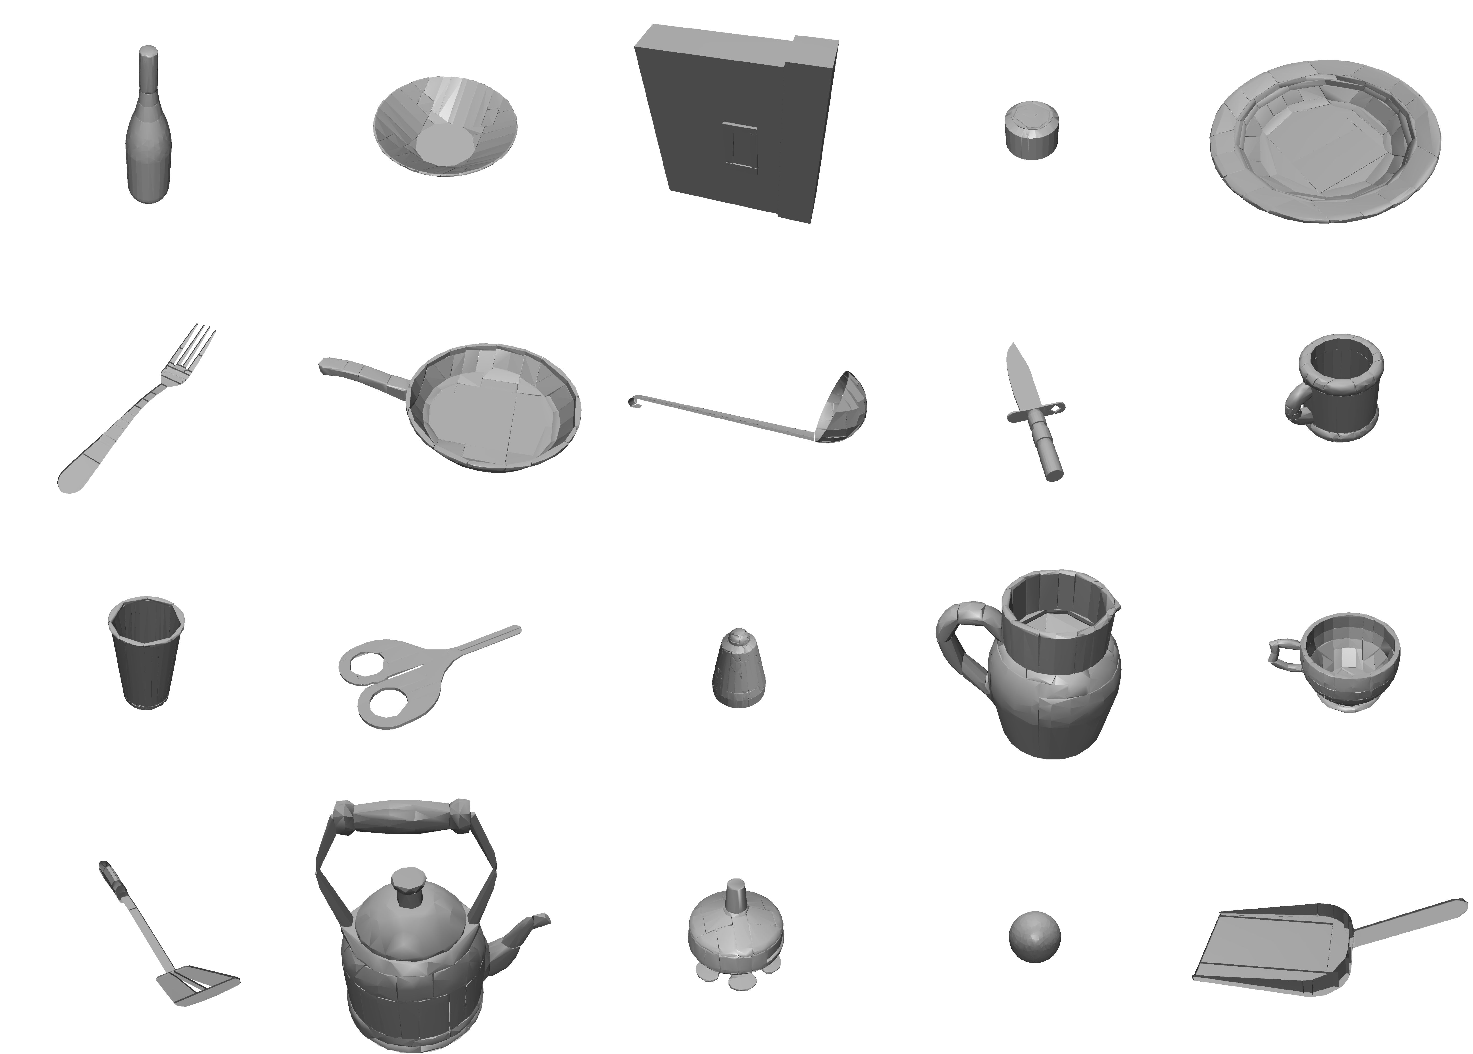
\includegraphics[width=\linewidth]{images/allObjects.pdf}
  \caption{Sample objects from all classes in the 3D model dataset.}
  \label{fig:allObjects}
\end{figure}
We trained our network on around 450000 grasps on 7000 distinct scenes, where each scene contains a random instantiation of one of the objects in the dataset with varying rigid body transformations applied, as well as friction and weight changes. The network was tested on 80000 grasps on 1200 scenes of unseen objects, as well as real robot experiments, as explained in Section \ref{section:experiments}. In order to make a direct comparison with Kopicki et al. \cite{kopicki2015ijrr}, we pick top grasps based on both the original ranking, as explained in Section \ref{section:generative}, and according to the predicted success probabilities by the network. 

We opted to use a grasp success prediction network due to the fact that the grasp generator function, explained in the previous chapter, provides alternatives of most intuitive types of grasps. A logical extension of this work would be to pair our learning algorithm with a grasp generator network, which we consider as future work.

Overall network architecture. VGG summary. Description of new layers. Representation of hand parameters, frames of reference, camera image conversion for VGG, trajectory of wrist and fingers.